%
% The Quantum Space Race
%

\subsection{The quantum space race}\index{Space race}\label{sec:quant_space_race_essay}

At the time of writing this book the world's first quantum-capable satellite was very recently launched into low-Earth orbit by Chinese scientists \cite{JWP}. The key capability of the satellite was to distribute entangled pairs of photons to ground stations thousands of kilometres apart. Using these entangled pairs, quantum key distribution was demonstrated, allowing theoretically unbreakable cryptography between the ground stations that no eavesdropper could compromise, guaranteed by the laws of physics.

However, entanglement distribution has many additional applications that are perhaps even more exciting than cryptography, most notably distributed quantum computation, enabling the world's future quantum computers to be networked into a virtual device with exponentially greater power than the sum of the parts.

The first generation satellite that was recently developed merely contained an entanglement source, and satellite-to-ground optical links via telescopes armed with laser tracking (Fig.~\ref{fig:first_gen_sat}). However, this prototype is strictly restricted to distributing entanglement between two ground stations, both simultaneously in line-of-sight of the satellite.

\begin{figure}[!htb]
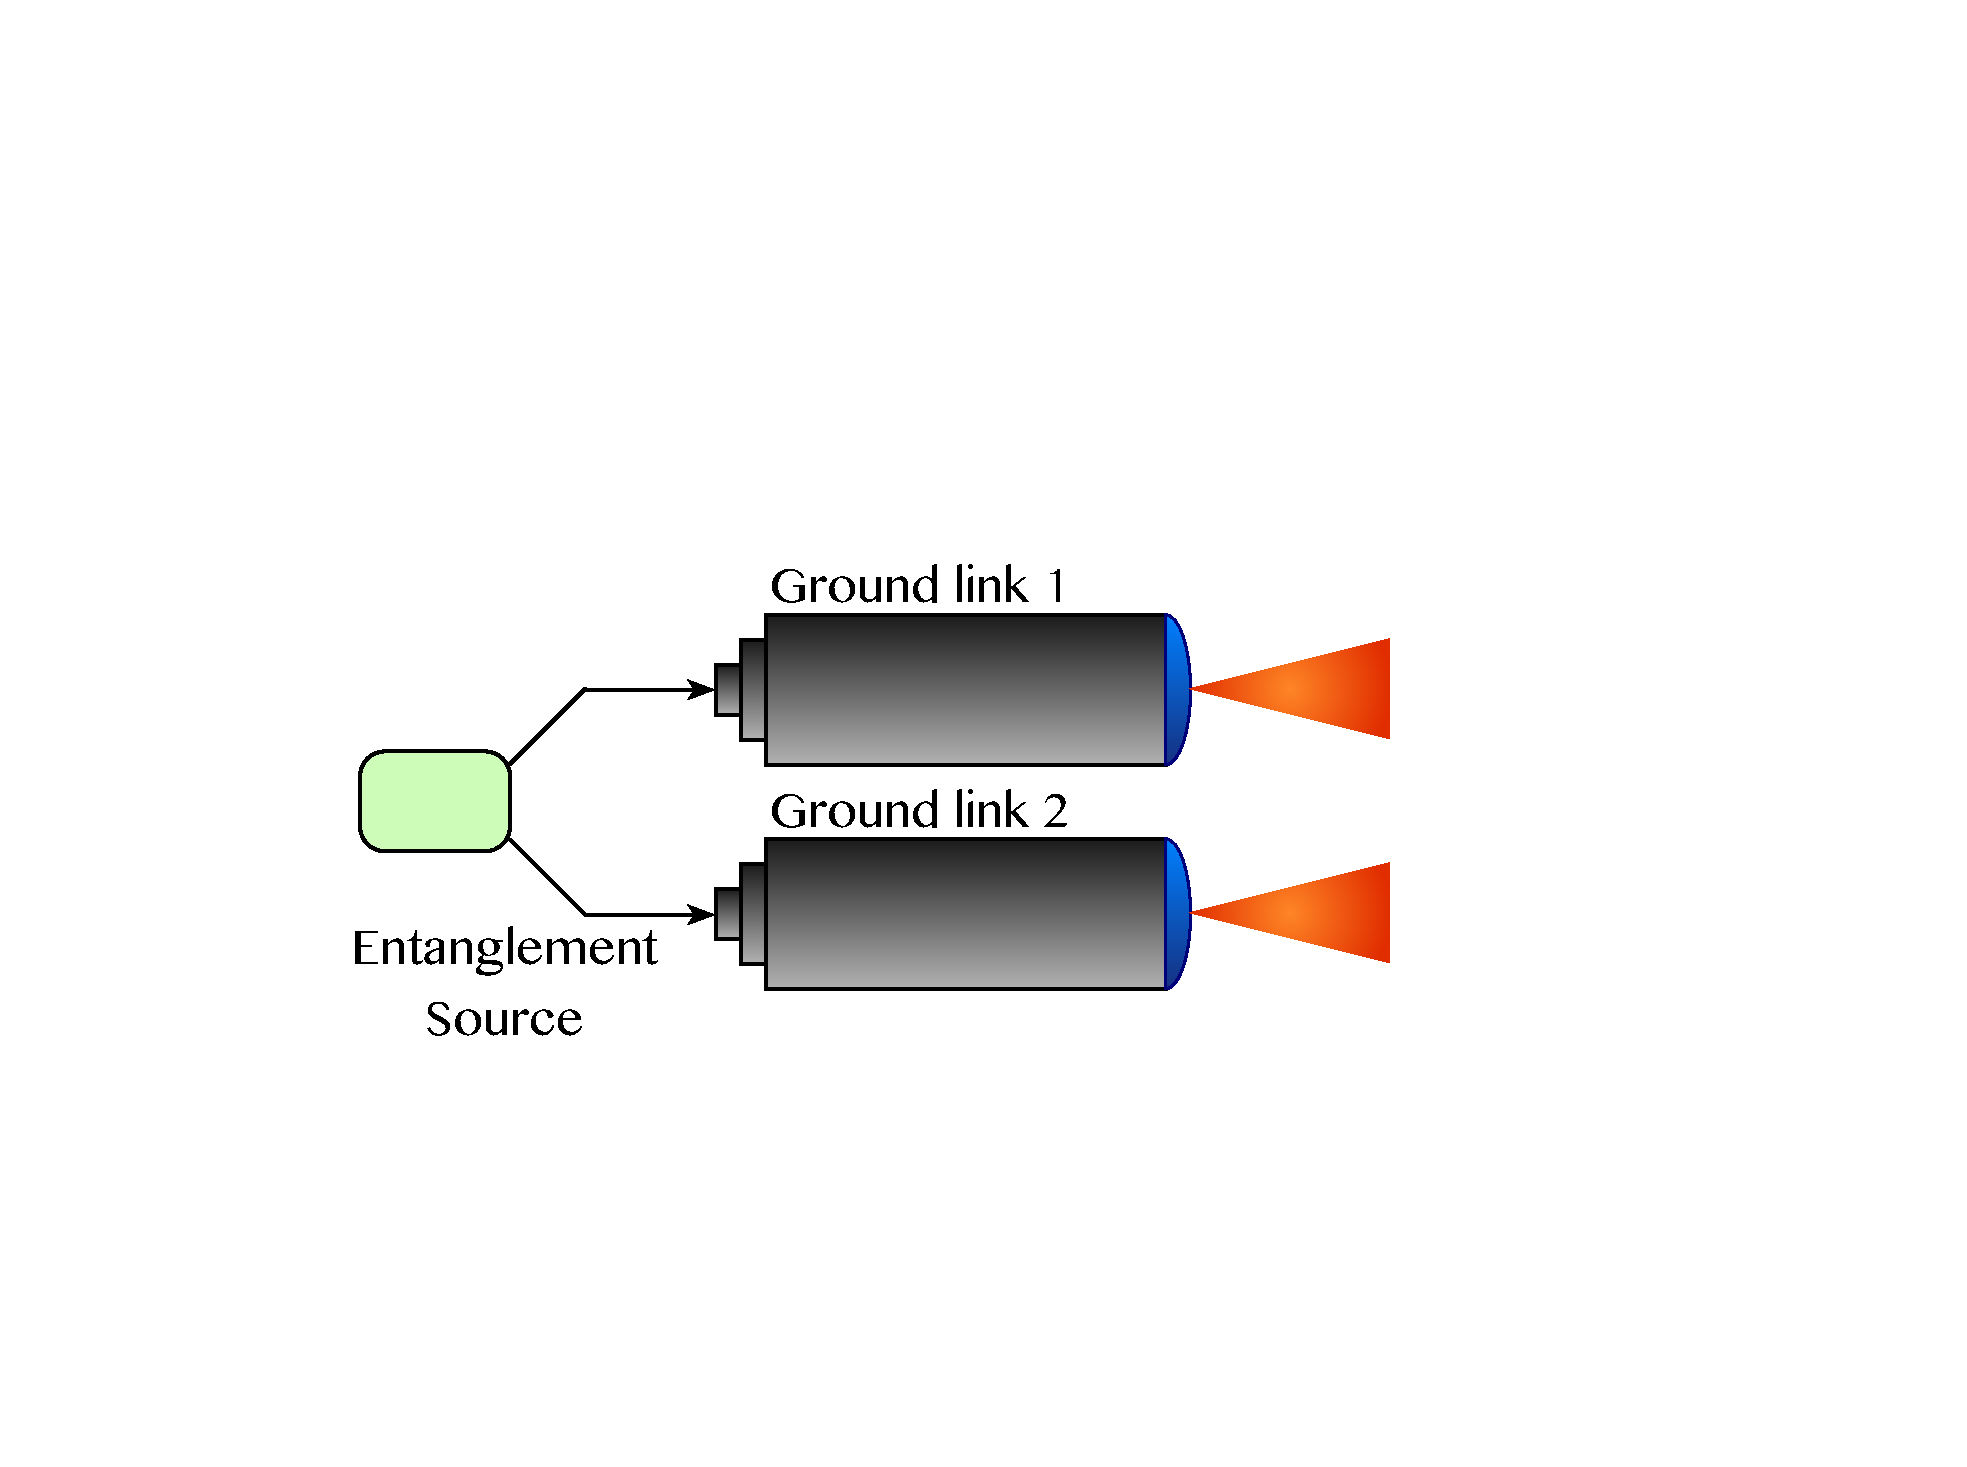
\includegraphics[width=0.47\textwidth]{first_gen_satellite}
\caption{First generation satellite for entanglement distribution. The on-board entanglement source couples to two telescopes, which lock onto independent ground stations using laser tracking.}\label{fig:first_gen_sat}	
\end{figure}

To facilitate a true global network, the next generation of satellites will need to form a constellation sufficiently dense that every point on the Earth's surface is always within line of sight of at least one satellite (Fig.~\ref{fig:sat_honeycomb}).

\begin{figure}[!htb]
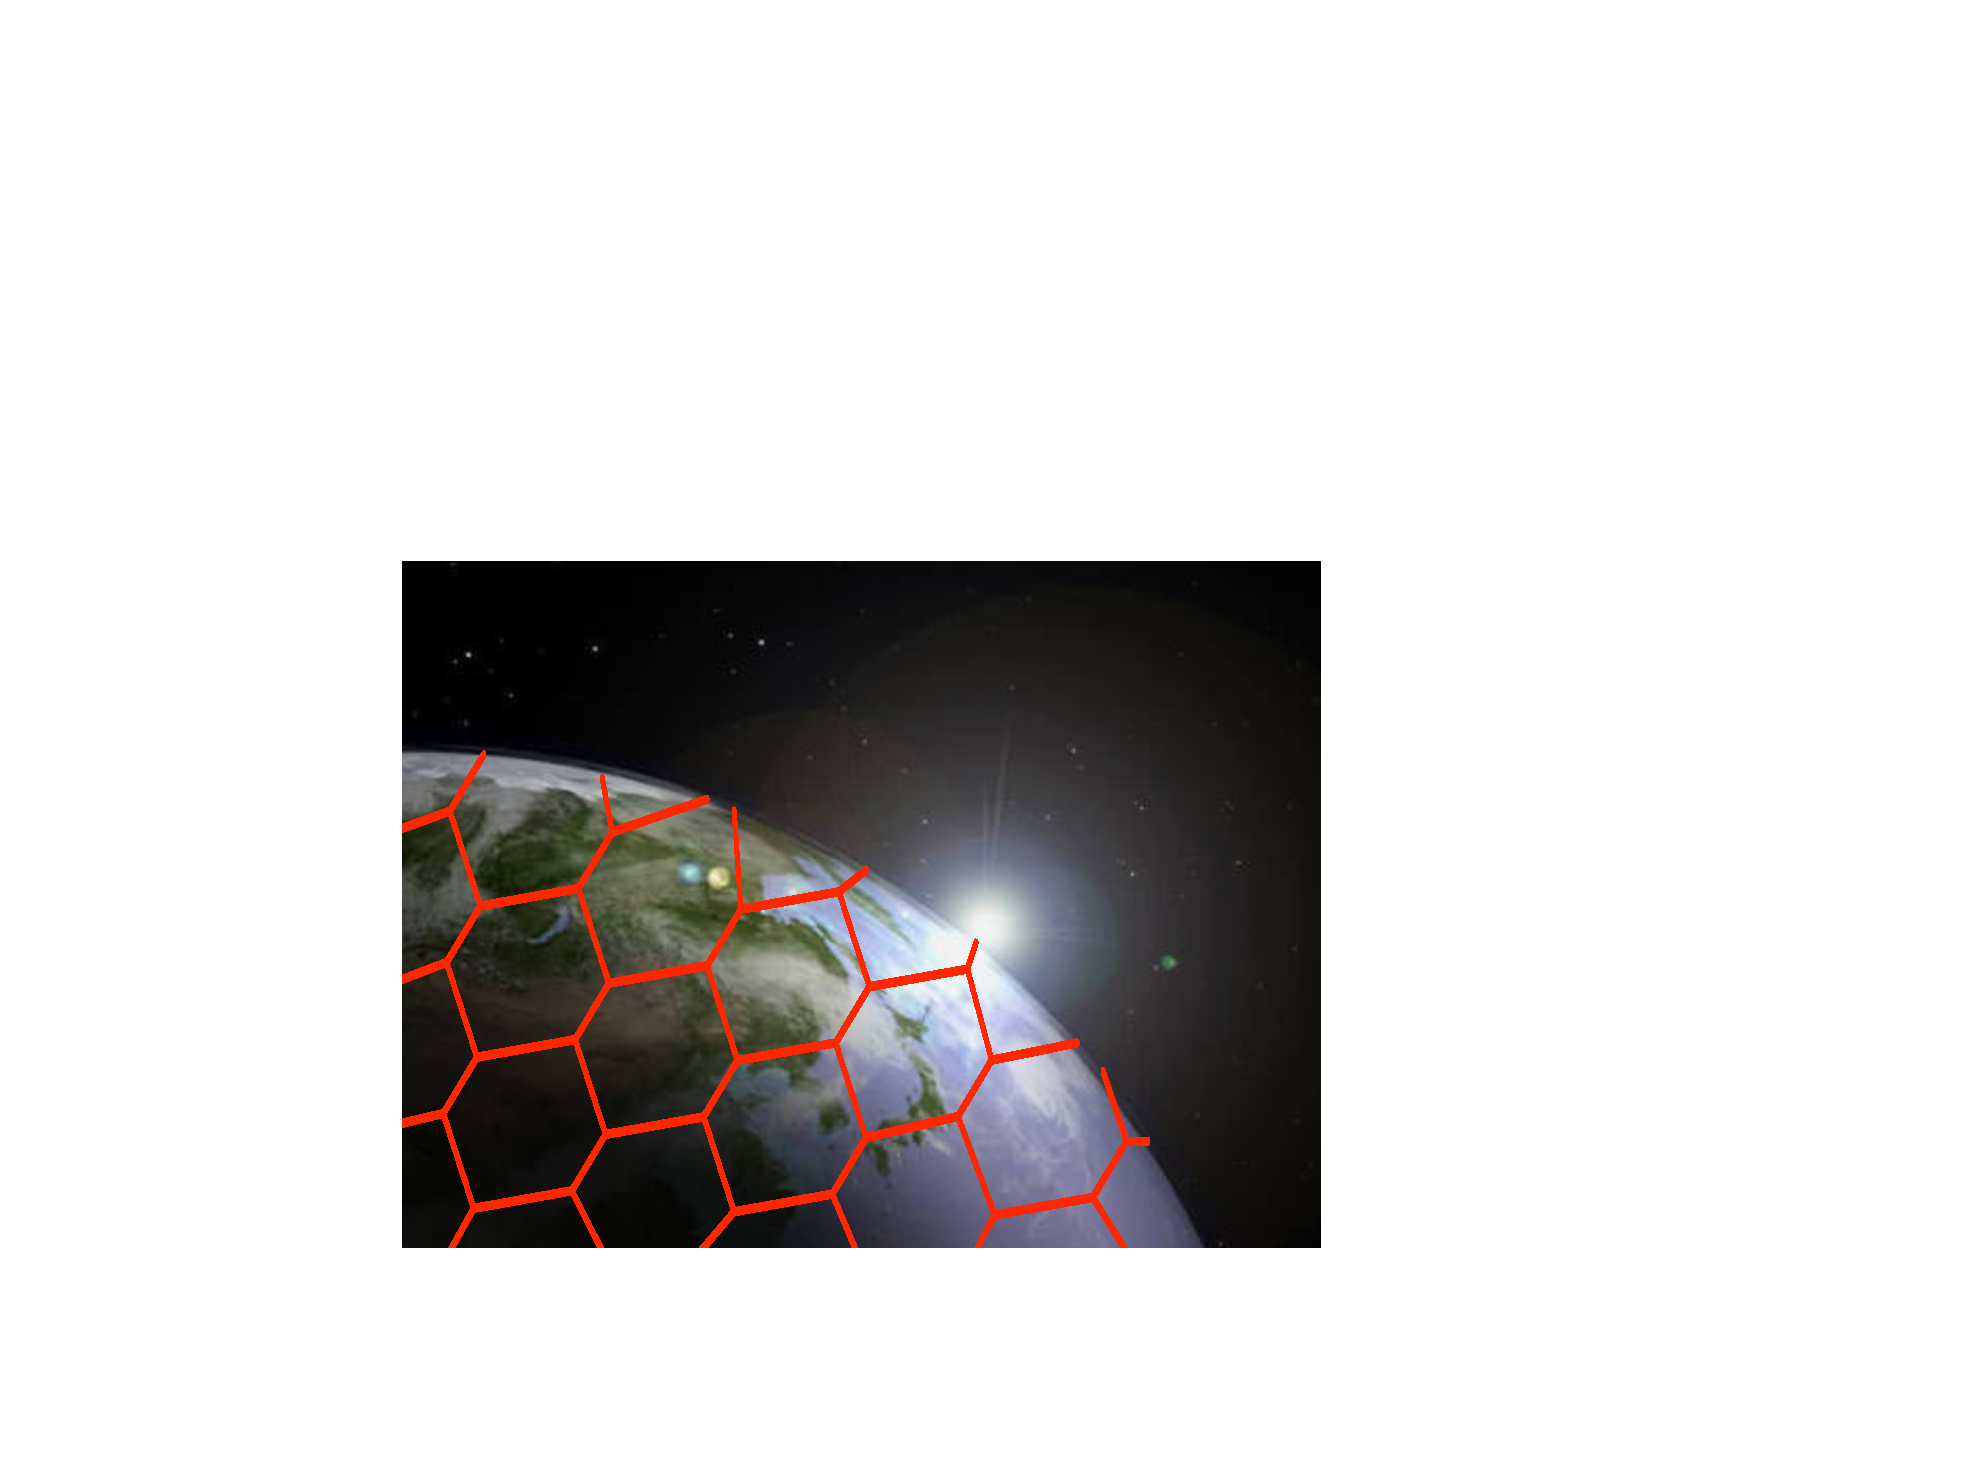
\includegraphics[width=0.47\textwidth]{satellite_honeycomb_lattice}
\caption{A honeycomb lattice is the lowest order two-dimensional lattice that could be employed to construct a satellite constellation network covering the Earth. Edges represent quantum communications channels, and their intersections are where the satellites reside. Such a network will require next-generation satellites with satellite-to-satellite links.}\label{fig:sat_honeycomb}	
\end{figure}

To enable a constellation, the satellites will need satellite-to-satellite links in addition to the satellite-to-ground links, such that they can relay the entanglement around the curvature of the Earth to overcome line-of-sight limitations. Additionally, they will need to do more than just prepare entangled states, but also perform entangling measurements, such that they can be configured as a quantum repeater network. A concept model for a next-generation satellite with these essential capabilities is shown in Fig.~\ref{fig:next_gen_sat}.

\begin{figure}[!htb]
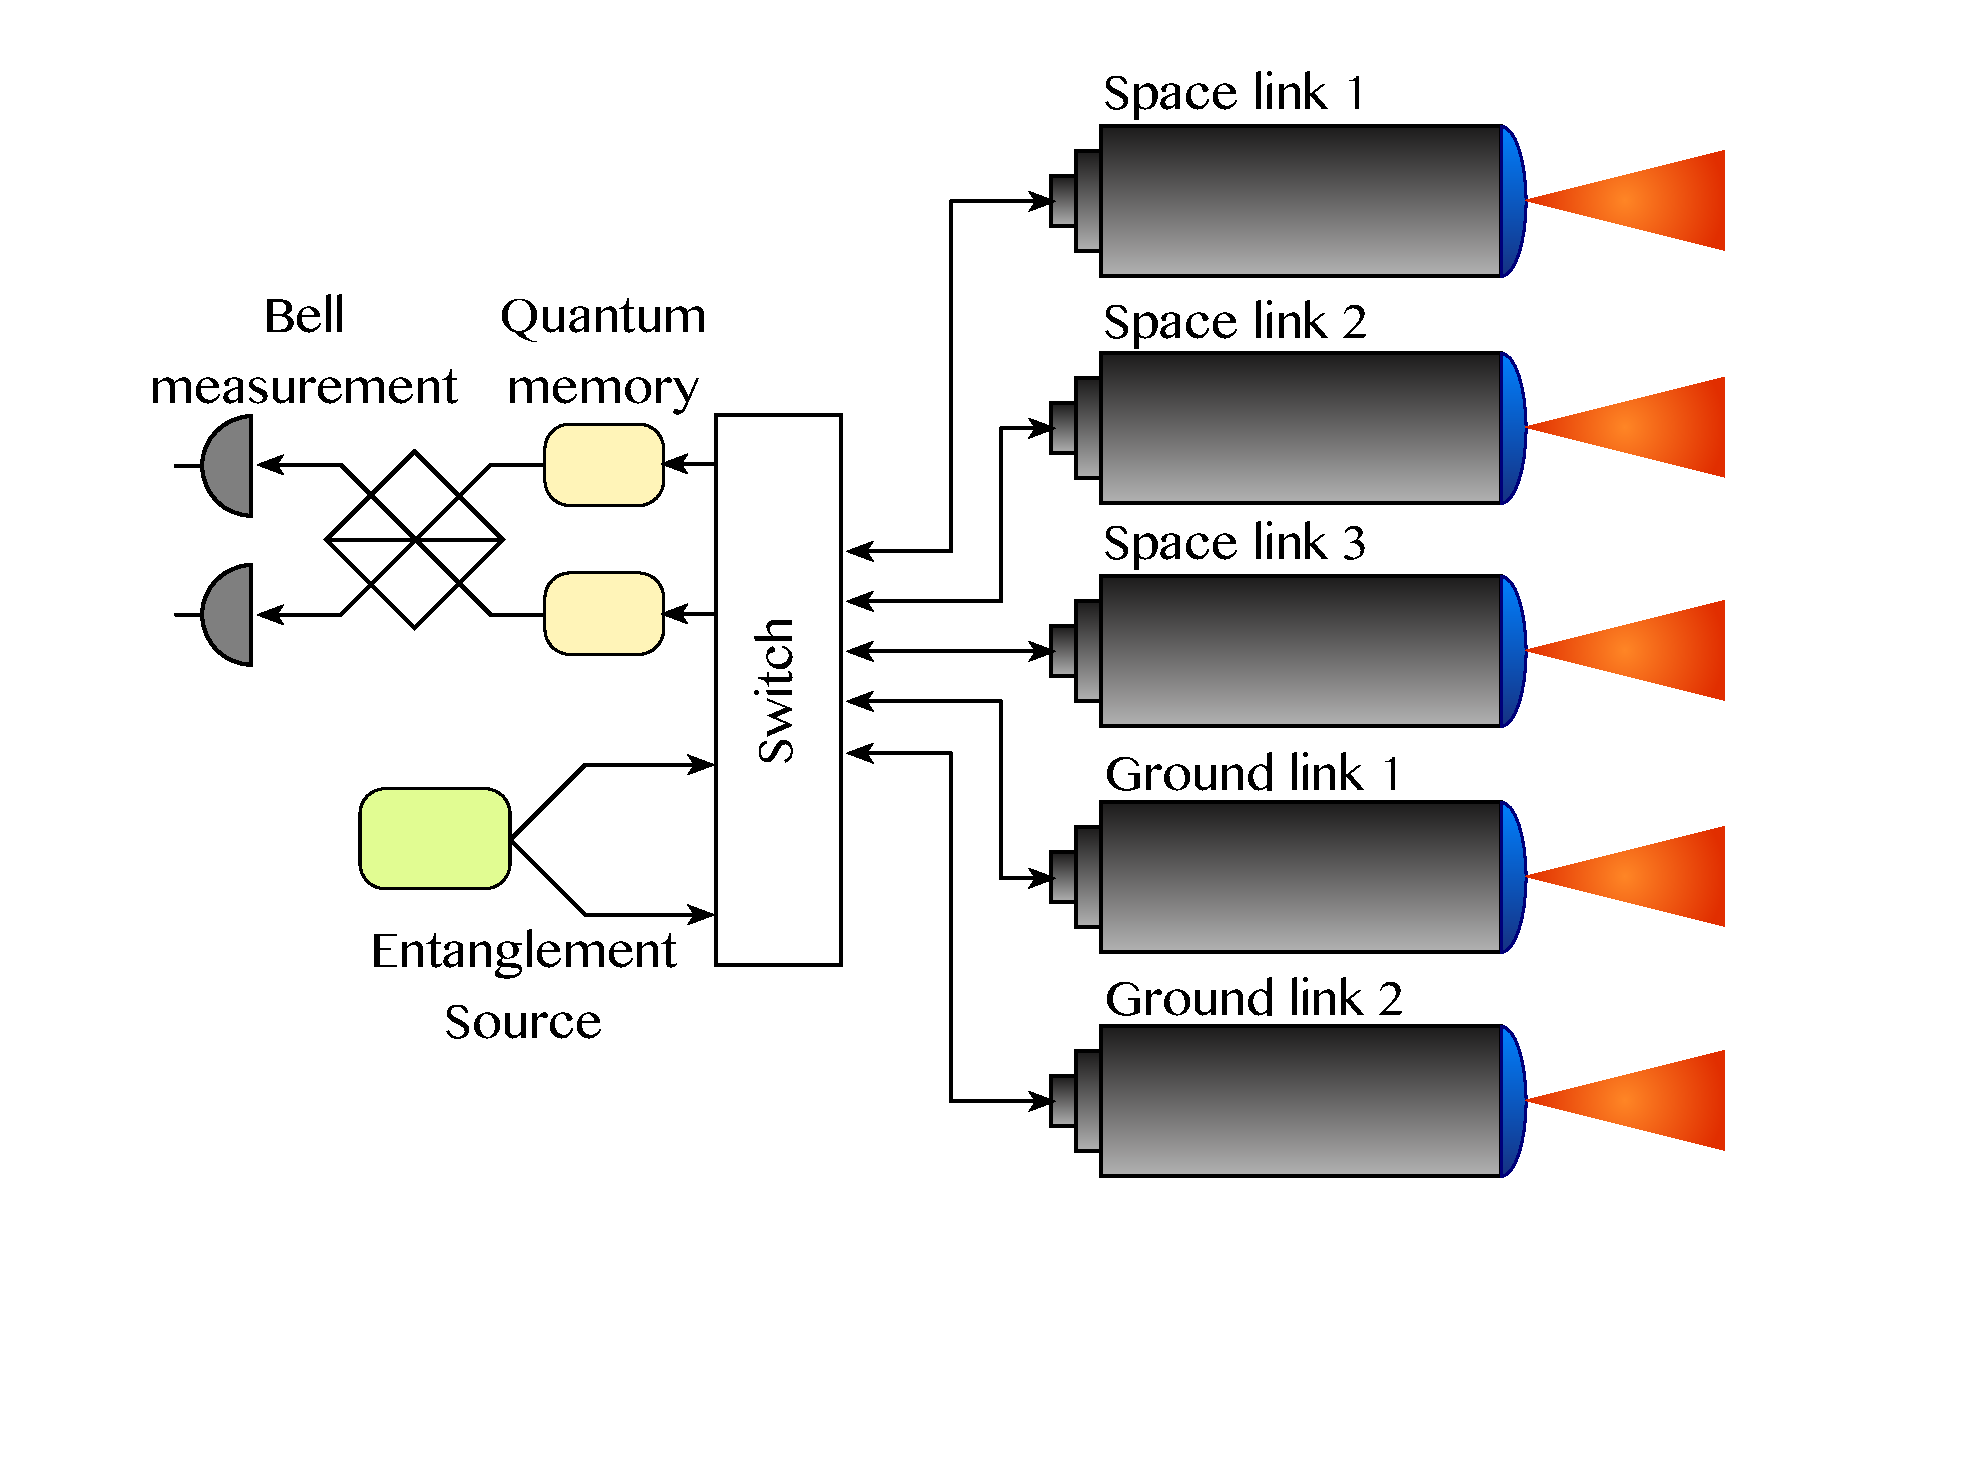
\includegraphics[width=0.47\textwidth]{next_gen_satellite}
\caption{A basic layout for how the next generation of quantum satellites might be constructed. Each satellite is capable of both entangled state preparation, as well as entangling measurements. There are three space links for communicating with neighbouring satellites so as to enable a honeycomb lattice configuration, as well as two ground links, as per the first-generation satellite. The switch at the centre must be universal to enable arbitrary pairs of telescopes to couple with either the entanglement source or entangling measurement. The quantum memories prior to the entangling measurement facilitate synchronising distinct photons with different arrival times such that they can interfere.}\label{fig:next_gen_sat}	
\end{figure}

While the next-generation satellite may appear only incrementally more complex than the first generation one, it is in fact far more technologically challenging. The main obstacle is that when performing entangling measurements, photons must arrive at the detector simultaneously. Obviously this is hard to enforce in space over long distances on fast-moving objects. Therefore quantum memories will be required, such that the first of two arriving photons is held in memory until the second one arrives, at which point it is read out from memory and the two photons are jointly measured. Unfortunately, such quantum memories are still very much in their infancy, and not reliable enough or of sufficient quality that they are ready for prime-time applications like a global space-based repeater network. It is unclear how far off these technologies are.

A global constellation network may require hundreds or thousands of individual satellites. The key to deploying such a network will be via economies of scale. We must design a single standardised satellite (for example along the lines of that shown in Fig.~\ref{fig:next_gen_sat}), rather than a variety of more specialised models, make it as minimalistic as possible, and then mass produce them on a large scale. With this approach we can hope for economical deployment of a true space-based point-to-point global network.

The Chinese have successfully launched and demonstrated the first quantum satellite. This marks the beginning of the quantum space race. Who will respond? For he who achieves a global network first will wield a huge competitive technological advantage in the upcoming era of the quantum internet and all its foreseeable and unforeseeable applications.